
\section{Example: Timing of algorithms} 
We usually think of random variables and
  associated density functions as being neat mathematical functions
  expressed as a function of the value and some parameters.  Mixture
  distributions are slightly more general versions of random variables
  and densities, but require more complex parameters.  The idea of a
  mixture is relatively simple.  To sample from one we have a two step
  random process.  We have $k$ simpler/regular densities and first
  select which one of these $k$ densities to sample from.  Having
  selected the component of the mixture, we generate a value from that
  density in the usual manner for that density, and then we have a
  value from the mixture distribution.  To specify a mixture we
  therefore have to specify the probability of selecting component
  $1$, $2$, $\ldots$, $3$ -- $(p_1, p_2, $\ldots$, p_k)$ -- and the
  form and parameters for each of the $k$ component densities.

  In this example, we focus on a mixture of $k$ Normals.  We will 
  write a function that returns $n$ sample values from a
  mixture of Normals.  It accepts three parameters: the number
  of sample values ($n$), the probabilities for sampling from each
  component ($p$ above), and an object representing the densities of
  the components.  For the latter, one might choose to use a $k \times
  2$ matrix to represent these parameters or a list of length $k$, each
  a named vector giving the mean and SD.  Alternatively one might use
  a list of functions to represent the densities with each having its
  own parameters stored within the function (e.g. using lexical
  scoping). This is the most general approach and allows one to have
  different types of distributions within the mixture.  One can create
  a new class to represent these also and provide methods for the
  class and to transform from one form to another.  You can choose for
  yourselves.

\begin{comment}
 You can also write the code to be more general
 to accept different types of base random variables and even allow
 different types of distributions within the same mixture, e.g. \alpha
 Normal (mu sigma2) + (1- \alpha) Exp(theta), but you don't have to! 
\end{comment}
 
 We examine two versions of the function
 in order to compare two algorithms.
 These are as follows.
 \begin{enumerate}
 \item The simplest way is to select which of the $k$ distributions to
   use for each of the $n$ points and then iterate over these n ``component
   identifiers'' for the distribution from which to sample and take a
   sample of size 1 from the corresponding density.
  
 \item An alternative approach is to generate the component identifiers
   for the $n$ deviates but then to determine how many observations
   are to be taken from each of the $k$ components.  Then iterate over
   the $k$ components and generate the appropriate number of random
   values from each of these.
 \end{enumerate}

 These two approaches produce the same results qualitatively, but 
 are different in terms of how fast they are.

 Generating the identifiers for the components is a sample from
 a multinomial distribution with parameters $p$.  You can use
 \SFunction{sample} to do this relatively easily in R.

  Let's start with a version that takes as input a matrix of
  parameters and vector of probabilities giving the proportions for
  which to sample each component.  The length of the vector should be
  the same as the number of rows as the matrix of parameters.
  We'll specify two here.
{\footnotesize{
\begin{verbatim}
M1 = matrix( c(0, 1, 0.1,
              10, 2, 0.3,
              -5, 1, 0.1,
               25, 2 ,0.3,
              -50, 5, 0.2), 
            nrow = 5, ncol = 3, byrow = TRUE,
            dimnames=list(seq(1:5),c("Mean","SD","Prob")))


M2 = matrix(c( -6, 1.5,
                0, 1.5,
                6, 1.5), , 2, byrow = TRUE)
\end{verbatim}
}}

  Now, before we go any further, let's look at the densities.
  To do this, we create a function that computes the density of the mixture
  at one or more values.  The following is one way to do it.  It
  accepts the probability vector and the parameter matrix of means and
  SDs for the mixture components, and the positions of $X$ at which to
  evaluate the density.  Then, it evaluates the density for each
  component at those points and adds them together using the
  proportions given in the vector \Svariable{p}.
\begin{verbatim}
dNormalMixture <-
function(x, p, params)
{
  tmp = cbind(params, p)

  rowSums(apply(tmp, 1, 
                  function(param) 
                     dnorm(x, param[1], param[2]) * param[3]))
}
\end{verbatim}
The actual implementation takes a short-cut: it adds the probability
vector as an extra column of the parameter matrix and then loops
over the rows, calling \SFunction{dnorm} for those values of x and
the specific parameters.  Adding the probabilities to the matrix
makes them available in each row.

Another way to do this is
\begin{verbatim}
dNormalMixture <-
function(x, p, params)
{
 rowSums(sapply(1:length(p),
                function(i)
                    dnorm(x, params[i, 1], params[i, 2]) * p[i]))
}
\end{verbatim}

You can now visualize the density of a mixture, e.g.
{\footnotesize{
\begin{verbatim}
curve(dNormalMixture(x, rep(1/3, 3), M2),
        -12, 12, ylab = "density")
\end{verbatim}
and
\begin{verbatim}
curve(dNormalMixture(x, c(.2, .5, .1, .1, .1), M1), 
           -65, 35, xlab = "density")
\end{verbatim}
}}


\begin{figure}[htbp]
\begin{center}
\leavevmode
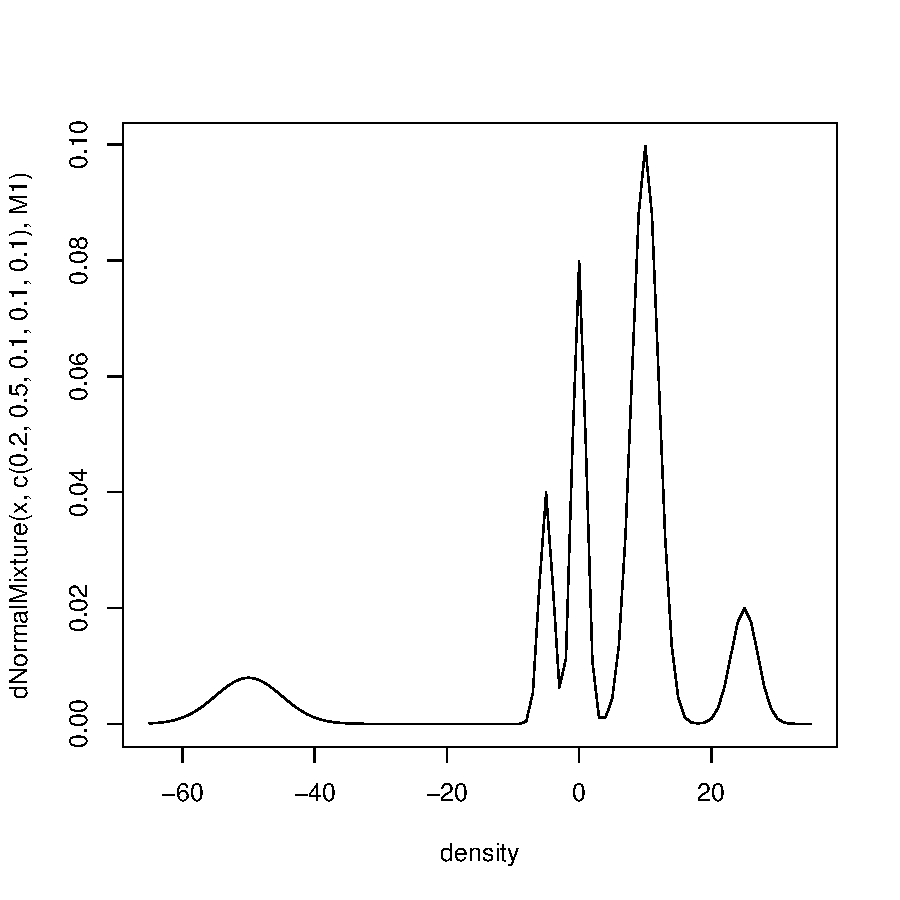
\includegraphics{RNG/images/mixtureDensity.pdf}
\caption{A density plot for a mixture of five normals with mixture
  probabilites, 0.2, 0.5, 0.1, 0.1, 0.1.}
\label{fig:mix5NormDensity}
\end{center}
\end{figure}


Let's now write a simple version of the function to generate
$n$ values from a general mixture of Normals.
Again, the important parameters are $n$, the number of values to
sample, $p$ the probability of selecting each of the components, and
the matrix of parameters for the components.  The mechanism we are
going to use is to generate a sample of size $n$ which identify from
which component to sample a Normal deviate.  When we have this vector
length $n$, we can loop over it and generate a single value from that
component of the mixture.  We have added two additional arguments to the
function definition below.  These are \SArg{whichComponent} and
\SArg{addComponentNames}.  The first of these allows the user to
explicitly specify the vector of component identifiers to sample for
each value. This has a default value which generates the sample if the
user does not specify it.  The reason we provide this is so that we
can explicitly control how many values to sample from each component.
This is useful when debugging, as we shall see.  The other argument --
\SArg{addComponentNames} -- merely instructs the code whether it
should identify which component was used to generate each value by
putting the index of the component as the element for that name.

{\footnotesize{
\begin{verbatim}
normalMixture <-
function(n, p, params,
         whichComponent = sample(1:length(p), n, replace = TRUE, prob = p),
         addComponentNames = TRUE)
{
  ans <- sapply(whichComponent,
                 function(i) {
                    par = params[i,]
                    rnorm(1, par[1], par[2])
                 })

  if(addComponentNames)
     names(ans) <- whichComponent

  ans
}
\end{verbatim}
}}
Hopefully the code should be reasonably self-explanatory given the
description above.

We can call it now with

\begin{verbatim}
x = normalMixture(10000, c(.3, .5, .2), M2)
\end{verbatim}

To verify that it is working, let's draw a histogram and superimpose
the  density.
\begin{verbatim}
hist(x, prob = TRUE, ylim = c(0, .14))
curve(function(x) dNormalMixture(x, c(.3, .5, .2), M2), 
       -12, 12, add = TRUE, col = "red")
\end{verbatim}
(We got the limits for the y-axis by trial and error.)

We should also try this for a different set of mixture inputs.
\begin{verbatim}
x = normalMixture(10000, c(.1, .2, .3, .2 , .2), M1)
hist(x, prob = TRUE, ylim = c(0, .15))
curve(dNormalMixture(x, c(.1, .2, .3, .2, .2), M1), 
       -60, 35, add = TRUE, col = "red")
\end{verbatim}


\begin{figure}[htbp]
\begin{center}
\leavevmode
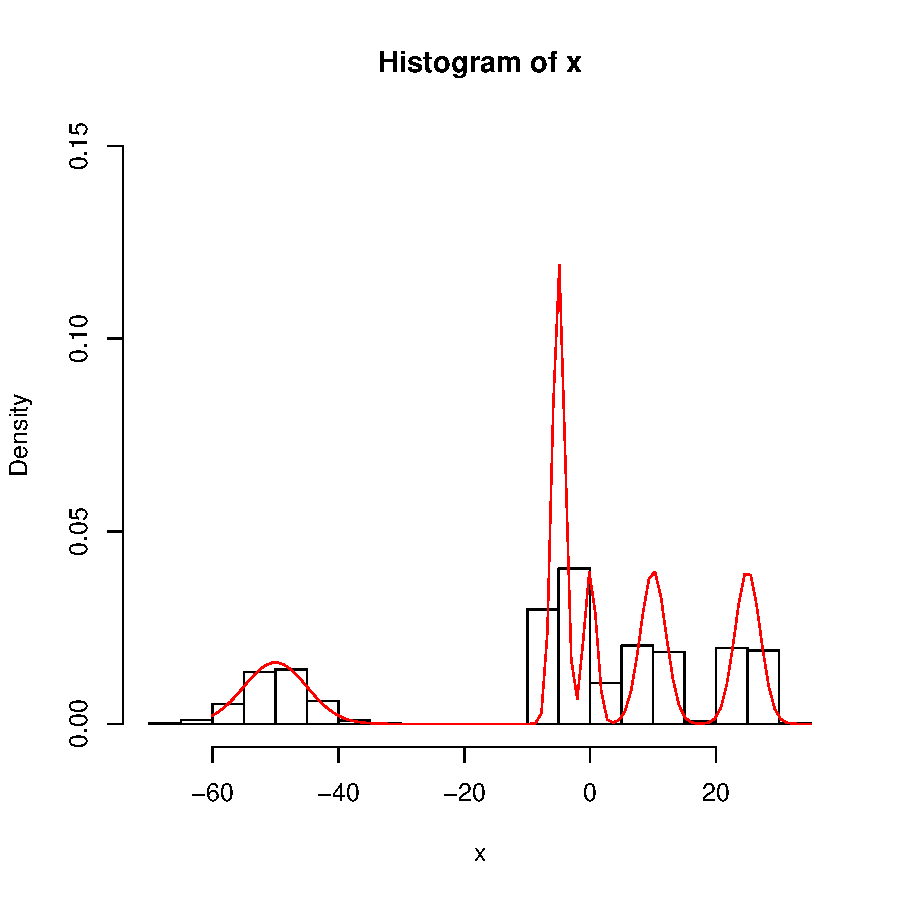
\includegraphics{RNG/images/mixtureSample1.pdf}
\caption{A histogram of a sample from a mixture of five normals with mixture
  probabilites, 0.2, 0.5, 0.1, 0.1, 0.1.}
\label{fig:mix5NormDensity}
\end{center}
\end{figure}

The shapes of the histograms are reasonably
consistent with the density curves, although
we probably need to either generate more
points or have a larger number of bins to get a better
visual fit.
\begin{verbatim}
hist(x, prob = TRUE, ylim = c(0, .15), breaks = 40)
curve(dNormalMixture(x, c(.1, .2, .3, .2, .2), M1), 
       -60, 35, add = TRUE, col = "red")
\end{verbatim}
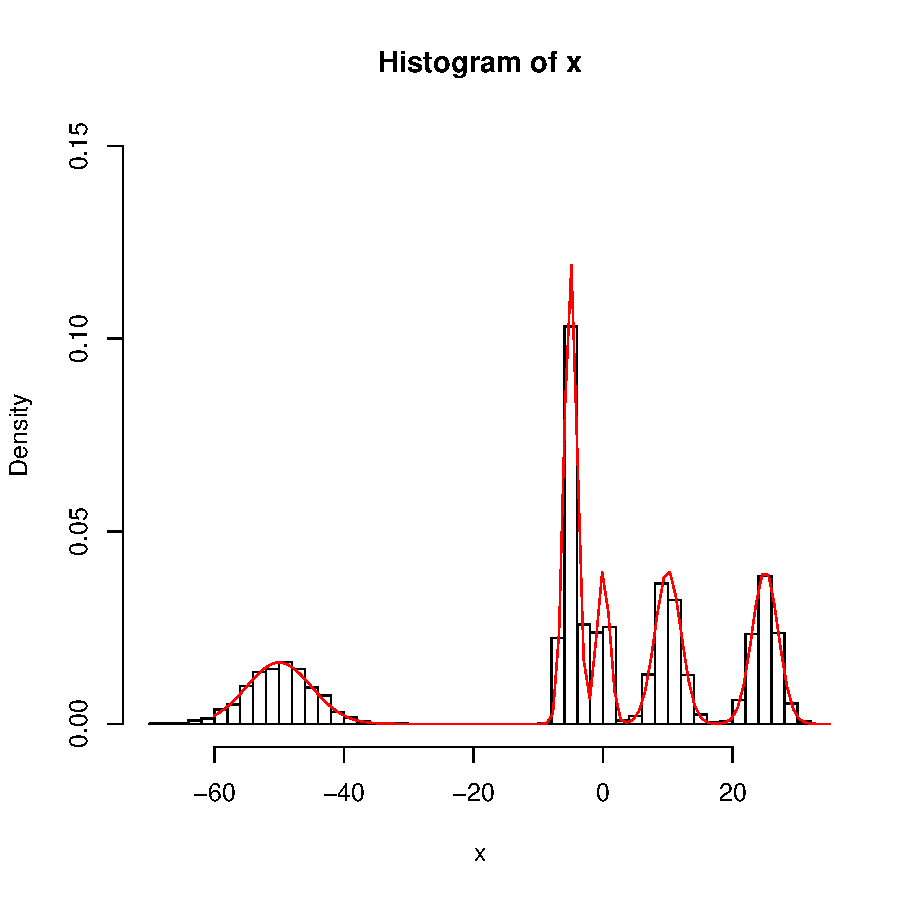
\includegraphics{RNG/images/mixtureSample1a.pdf}

Now, let's write the second and hopefully faster version of the
\SFunction{normalMixture} function.  In this version, we essentially
determine how many values -- $n_i$ --- we should sample from each
component $i$ and then generate that number in a single call to
\SFunction{rnorm}.  There are two ways to generate these counts for
each component. One is to take a sample as we did above of size $n$
from the set 1, 2, $\ldots$, k and then use \SFunction{table} to
compute the counts in each category/component.  Alternatively, we can
use \SFunction{rmultinom} to generate a single sample of $n$ values
from a multinomial distribution.
For example, 
\begin{verbatim}
rmultinom(1, 10, c(.2, .5, .3))
     [,1]
[1,]    0
[2,]    7
[3,]    3
\end{verbatim}
divides 10 into 3 groups with the corresponding probabilities of each
element being in that group.

Note that the first component had no values but was listed
in the answer.
Using \SFunction{table}, this does not happen.
For example, 
\begin{verbatim}
table(sample(1:3, 10, replace = TRUE,
      prob = c(.01, .5, .49)))
2 3 
5 5 
\end{verbatim}
has no entry for 1.
This difference makes the how we sample from the components
just a little different for the two approaches.

The idea is quite simple for \SFunction{rmultinom}.
We get the counts for the components and loop
over these and generate the $n_i$ values.
We need to index both the counts vector and 
the parameter matrix rows.
So we loop over the row indices
with \Sexpression{seq(along = counts)}
which is equivalent to \Sexpression{1:length(counts)}
but works well when counts has no elements.
{\footnotesize{
\begin{verbatim}
normalMixture.faster <-
function(n, p, params)
{
  counts <- rmultinom(1, n, p)

   # loop over 1:length(p) and generate n_i values from 
   # each component.
  l = lapply(seq(along = counts),
              function(i) {
                 rnorm(counts[i], params[i, 1], params[i, 2])
              }) 

  unlist(l)
}
\end{verbatim}
}}
Note that at the end of the \SFunction{lapply} call, we end up with a
list and we don't want to simplify it with \SFunction{sapply}. This is
because each element in the list will typically have different size.
So at the end of the function we call \SFunction{unlist} to unravel
all the values into a single vector.

The version using \SFunction{sample} and \SFunction{table}
is similar and given by
{\footnotesize{
\begin{verbatim}
normalMixture.faster <-
  #
  #  The faster way to generate n values from a mixture
  #  by counting the number in each group and then 
  #  generating that number for each group in a single call.
  #
  #
function(n, p, params, 
          counts = table(sample(1:length(p), n, 
                                replace = TRUE, prob = p)),
                         addNames = TRUE)
{
  ans <- unlist(lapply(seq(along = counts),
                 function(id) {
                   par = params[as.integer(names(counts)[id]),]
                   rnorm(counts[id], par[1], par[2])
                 }))

  if(addNames)
     names(ans) <- rep(names(counts), counts)

  ans
}
\end{verbatim}
}}
The primary differences between here and the one above is that we have
added the extra arguments \SArg{counts} and \SArg{addComponentNames}
as we did earlier.  And the loop in the \SFunction{lapply} has to do
some apparently more complex indexing to get the parameters for the
particular parameter.  This is because the position in the
\Svariable{counts} variable does not necessarily correspond to the row
of the component in parameter matrix.  Some of the
categories may have no elements and be dropped from the frequency
table, so we turn the name of the element of \Svariable{count} from a
string to a row index in the parameter matrix.  Again, we add names to
identify the component if they are requested.

We check the histograms as above.  In addition to this check, however,
we can also compare the output from each function to each other.  We
can use a Q-Q plot for this since the two distributions of numbers are
supposed to be the same.

\begin{verbatim}
x1 = normalMixture(10000, 
       c(.1, .2, .3, .2 , .2), M1)
x2 = normalMixture.faster(10000, 
       c(.1, .2, .3, .2 , .2), M1)
qqplot(x1, x2)
\end{verbatim}


\begin{figure}[htbp]
\begin{center}
\leavevmode
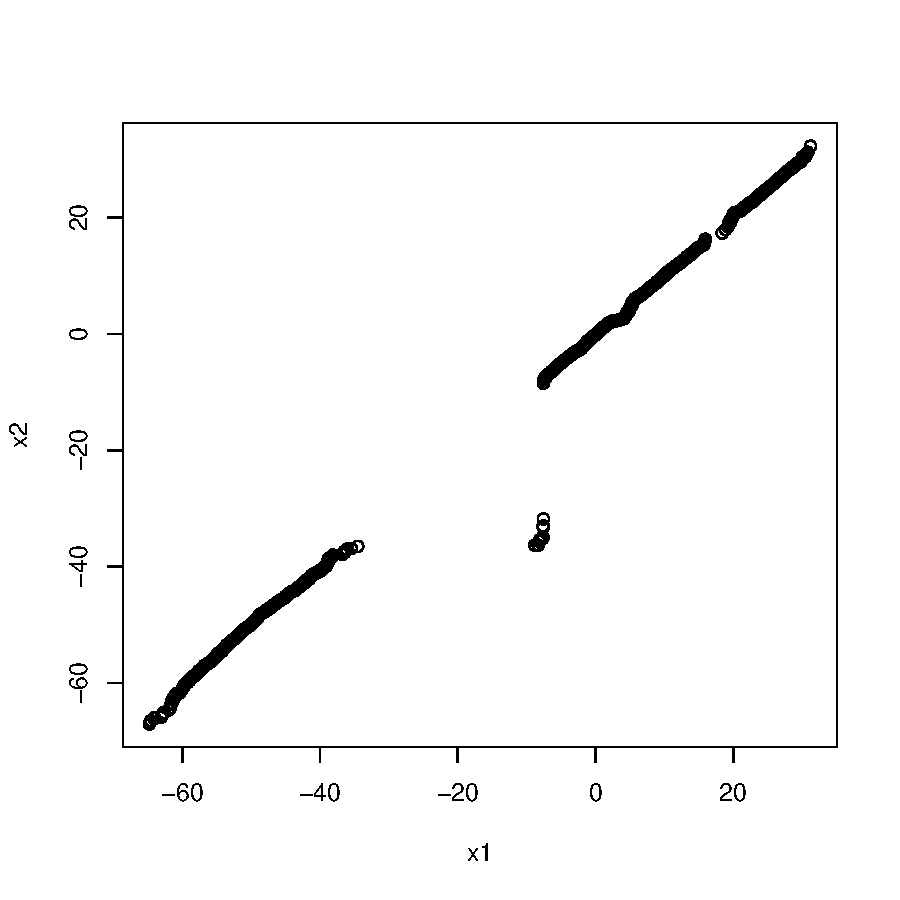
\includegraphics{RNG/images/algorithmBasicQQplot.pdf}
\caption{A quantile-quantile plot for samples from the two methods for
  generating observations from a mixture of five normals.}
\label{fig:mix5NormDensity}
\end{center}
\end{figure}

This is supposed to yield a straight line up to sampling variability.
And with $10,000$ observations, it should be very good.  However, we
see major departures from the line.  The primary trend is definitely a
straight line as we expect, but there are major ``bumps''.  After a
bit of investigation, we can figure out what is causing these and why
the Q-Q plot appears erroneous. And then we can conclude that the
algorithms are really giving qualitatively similar results.

Let's take a look at the actual values coming from each algorithm.  We
want to add these to the Q-Q plot and it would be good to color code
them base on which component they were sampled from.  To do this, we
need to be able to determine the component for each value.  This is
what the \SArg{addComponentNames} argument does in our two functions;
it adds the component identifiers as names for the  result vector, 
identifying each element's component.
The function \SFunction{showQQ} and \SFunction{drawRug} below 
draws the Q-Q plot with this additional information.
{\footnotesize{
\begin{verbatim}
showQQ =
  #
  # Draws a QQ plot of the two data vectors
  # and assumes they have names identifying
  #
function(x, xx, pch = "o", showLine = TRUE)
{  
  qqplot(x, xx, pch = pch, pty = "s") # force square aspect ratio.
  if(showLine)
     abline(a = 0, b = 1, col = "red")

  drawRug(x)
  drawRug(xx, 3)
  drawRug(xx, 2)
}

drawRug =
  #
  # Plot the data for the different groups identified by their names.
  #
function(x, side = 1) {
       k = levels(factor(names(x)))
       colors = rainbow(length(k))
       for(i in seq(along = k))
         rug(x[names(x) == k[i]],  col = colors[i], side = side)
}
\end{verbatim}
}}

Now, we can use this to see more information about our plot.
\begin{verbatim}
showQQ(x1, x2)
\end{verbatim}
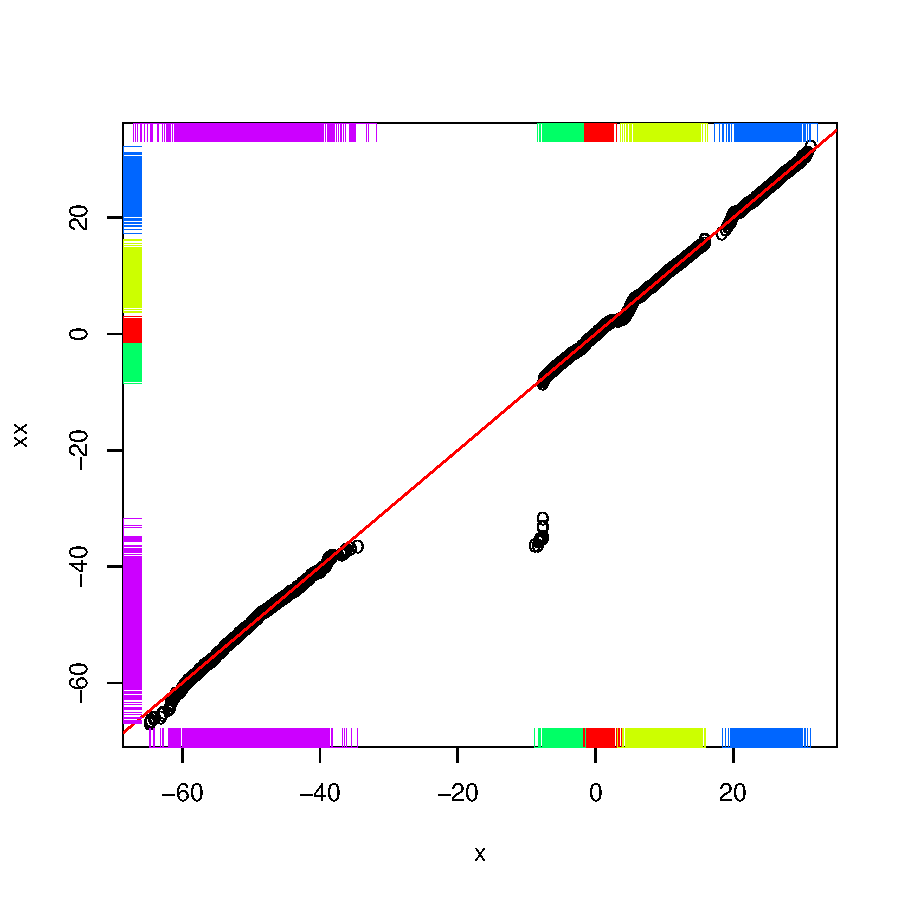
\includegraphics{RNG/images/algorithmRugQQ.pdf}

Hopefully, you can see that the bumps occur at the break points
between two components, on either the horizontal or vertical axis.
Specifically, look at the lower-left corner of the plot.  There is a
big departure from the line, with a couple of points below and to the
right of the line.  If we see which components these correspond to, we
see what is the problem.  On the horizontal axis, these points are
from the second component (green), but on the vertical axis, they are
from the first component (purple).  Since these two components have
very different typical values, the minimum of the second is nowhere
close to the maximum of the first.  And so the pairs of points are way
off the straight line we expected.  This is good explanation of why
the bumps appear.  It also tells us that the problem is that because
of the randomness in the sampling process, there are fewer
observations from component 1 in the first set of data
(\Svariable{x1}) than in \Svariable{x2}.  It is this difference that
really causes the bumps.  If we force them to have the same number in
each component, then we should get a Q-Q plot much closer to the
expected straight line.  We can do this by specifying which components
to sample from in each algorithm using the \SArg{which Component}
argument added to the functions.

\begin{verbatim}
components = sample(1:5, 10000, prob = c(.1, .2, .3, .2 , .2), replace = TRUE)
x1 = normalMixture(10000, c(.1, .2, .3, .2 , .2), M1,
                         whichDist = components)
x2 = normalMixture.faster(10000, c(.1, .2, .3, .2 , .2), M1,
                           counts = table(components))
\end{verbatim}
Now, the Q-Q plot of these two vectors is a straight line,
with  breaks where there are no values.

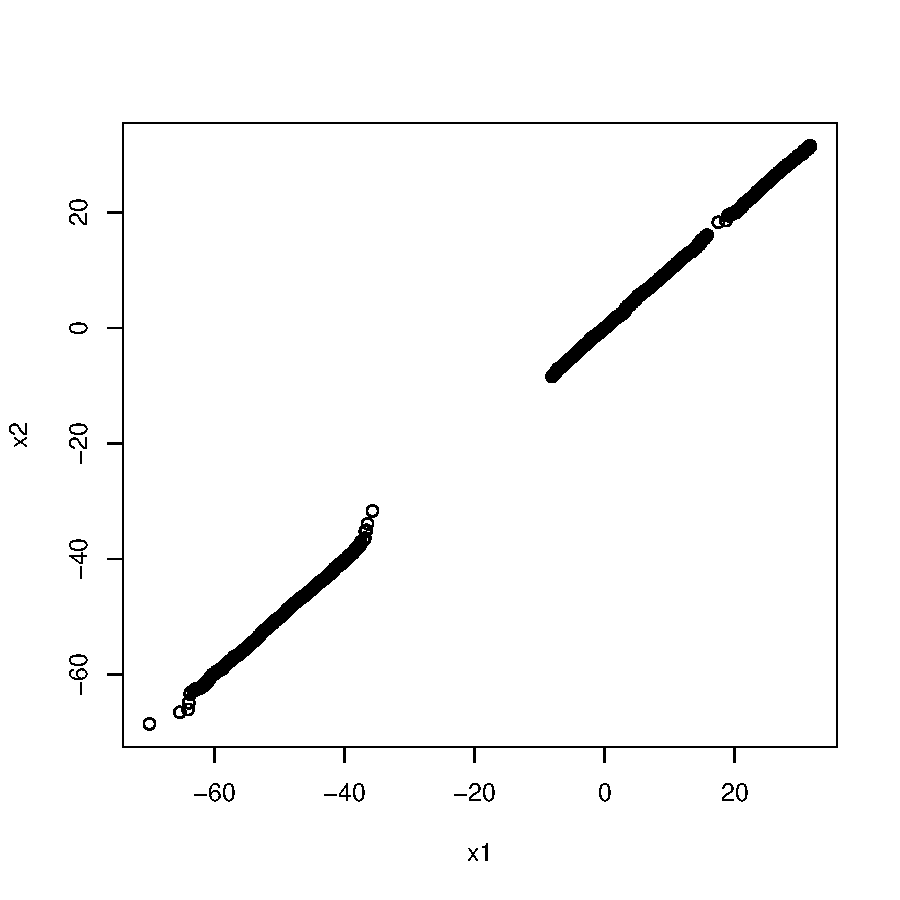
\includegraphics{RNG/images/SimpleQQEqualCount.pdf}

Using \SFunction{showQQ}, we can see that the components match up
in this case and there are no bumps.

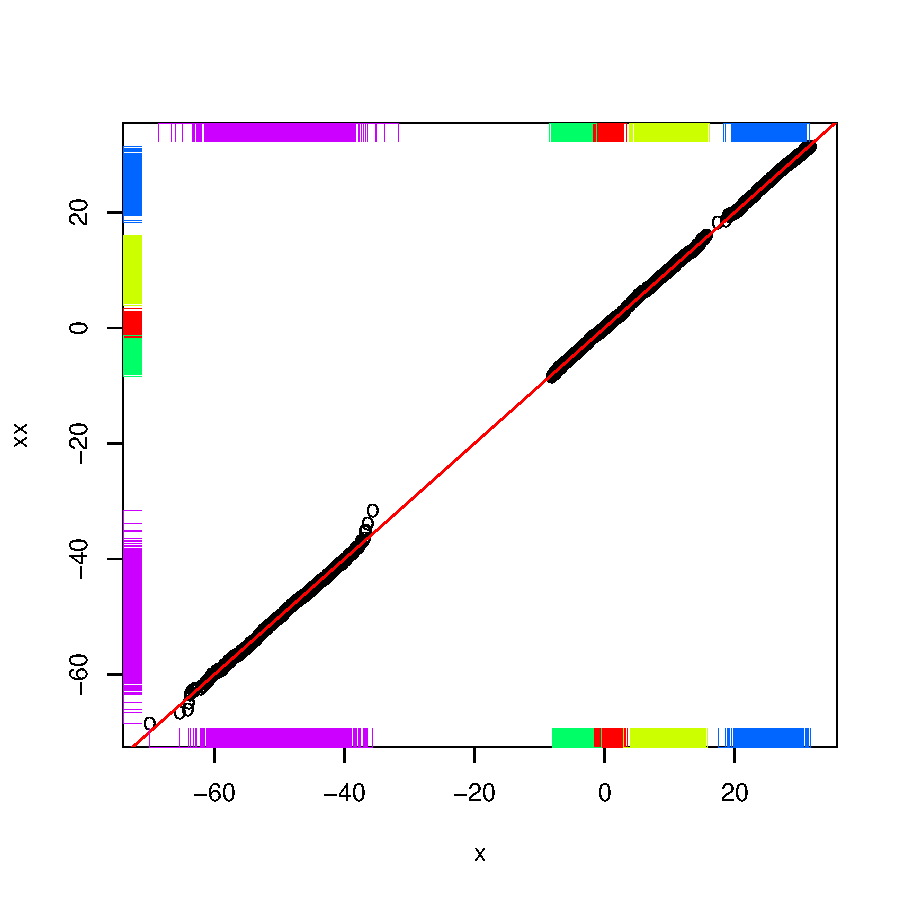
\includegraphics{RNG/images/QQEqualCount.pdf}

Now, we can move on to comparing the speed of the two algorithms for
different sample sizes.  We will look at this for $5$ different sample
sizes, $1, 10, 100, 1000, 10000$.  Then we loop over the two functions
and for each of these, we loop over the sample sizes.
Then, for each sample size and function pair, we perform the
random sample $11$ times and count the time for each.
{\footnotesize{
\begin{verbatim}

# Can do this in two separate pieces of code, but really a repetition.
# and if one needs to change one, then need to change the other.
# e.g. adding system.time.
sampleSizes <- c(1, 10, 100, 1000, 10000)
names(sampleSizes) <- sampleSizes

# Choose prime numbers (2, 5, 11) so that we can identify the
#  dimensions in the result if they are collapsed.

tt <- lapply(list(basic = normalMixture,
                   counts = normalMixture.faster),
        function(f) {
              lapply(sampleSizes,
                      function(n) {
                         sapply(1:11, function(i) {
                            system.time(f(n, c(.3, .2, .5), 
                                          matrix(c(.2, .1, 
                                                   .5, .3, 
                                                   .8, 1), ,
                                                  2, byrow = TRUE)))
                       })
                     })
             })



# Note that this doesn't work in S-Plus as n is not in 
# the scope of the inner function.

 # Just look at elapsed time.
elapsedTimes <- sapply(tt, function(f)  
                            sapply(f, function(m) mean(m[3, drop = FALSE])))

matplot(sampleSizes, elapsedTimes, type = "l",
            xlab = "Sample Size", ylab = "seconds", 
            main = "Elapsed time for two algorithms")

legend(400, .9*max(elapsedTimes), c("basic", "counts"), 
        col = 1:2, pch = as.character(1:2))
\end{verbatim}
}}
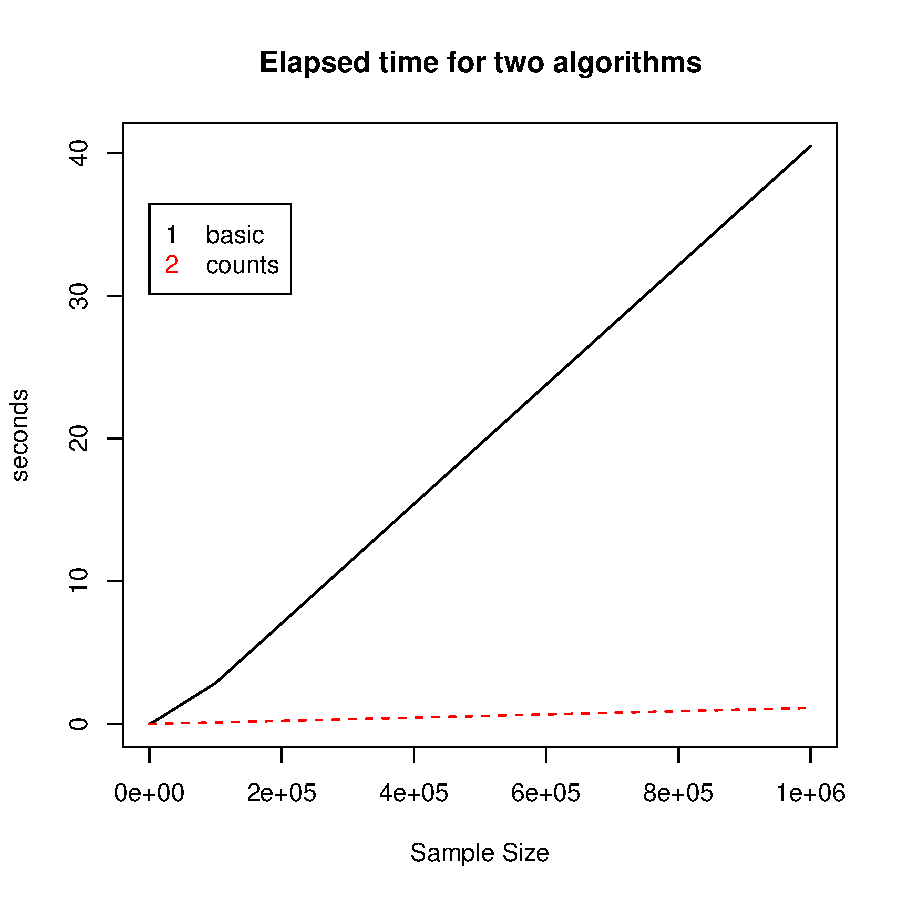
\includegraphics{RNG/images/algorithmTimes.pdf}
We see that there is a large difference in run-times as $n$ increases.
The second algorithm is much faster.
As we go to larger $n$

Any oddity for $n = 1$ is caused by the fact that we cannot measure
very short runs accurately. Rather than taking the mean of
$k$ runs for $n = 1$, we should take the total time
for $k$ runs and divide it by $k$ when the time being measured
is very small.


The moral to take away from this exercise is that the naive way of
doing things is a good one to work on first and use as a validation
test; but it is often appropriate to find a vectorized form of the
function in order to make it more efficient, but only if the time
spent making the code faster is less than the amount of time saved in
running the more efficient code!


